% !TEX root = ../msc_thesis.tex

\chapter{Project Website}
  \label{ap:Website}

  \section{Consent Form}
    \label{aps:consent}
    You are being invited to participate in this academic study. This study is being done by Vasilis Gerakaris as part of a MSc Project under the supervision of professor \href{http://homepages.inf.ed.ac.uk/da/}{David Aspinall} for the \href{http://www.ed.ac.uk/}{University of Edinburgh}.

    If you agree to take part in this study, you will be asked to complete an online survey/questionnaire after completing a mock registration process.

    The selected partial password (memorable information) will stored in cleartext (not encrypted) in our database. In simple terms, this means that we will be able to see the password you have selected.

    While we do not retain any identifying information other than your Worker ID, we strongly suggest that you do \textbf{not} select a password you already use on other accounts.

    We believe there are no known risks associated with this research study; however, as with any online related activity the risk of a breach of confidentiality is always possible. To the best of our ability your answers in this study will remain confidential. After the experiment has concluded and statistical results have been generated, all stored information will be permanently deleted.

    If you have questions about this project or if you have a research-related problem, you may contact the researcher, Vasilis Gerakaris at the following email address: \texttt{s1568962@sms.ed.ac.uk}

    By clicking ``Accept'' below you are indicating that you are at least 18 years old, have read and understood this security notice and agree to participate in this research study. Feel free to print a copy of this page for your records.

  \section{Home page}
    \label{aps:homepage}
    \begin{figure}[H]
      \makebox[\textwidth][c] {
        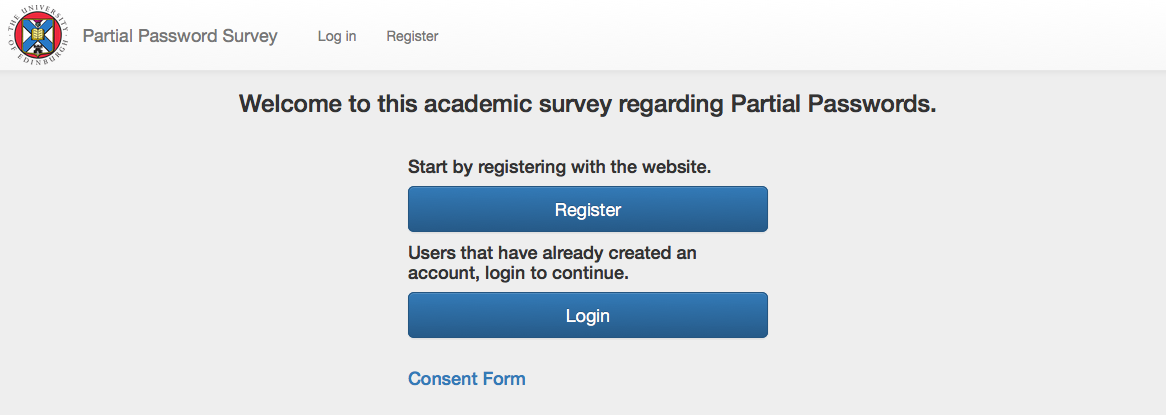
\includegraphics[width=1.3\textwidth]{Images/0-home}
      }
      \caption{Homepage}
      \label{fig:home}
    \end{figure}

  \section{Introduction}
    \label{aps:intro}
    Imagine that the following is part of the registration process for a bank. The memorable information you select will be used to access online banking services. You will be asked to use this memorable information in a few days to log in again, so it is important that you remember it. Please take the steps you would normally take to remember and protect this information as you would normally protect the ones for your bank account. Behave as you would if this were your real banking credentials.\\

    Do not select a password you already use on other accounts, as I will be able to see them (they are stored in cleartext, not encrypted).

  \section{Registration page}
    \label{aps:registration}
    \begin{figure}[H]
      \makebox[\textwidth][c] {
        \begin{subfigure}[t]{0.4\textwidth}
            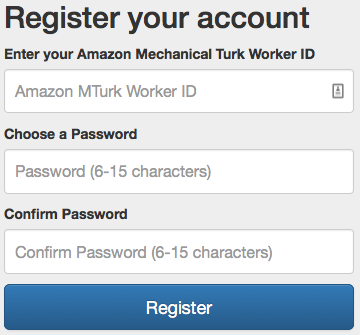
\includegraphics[width=\textwidth]{Images/1-register-nostr}
            \caption{Without strength meter}
            \label{fig:reg-nostr}
        \end{subfigure}
        ~ %add desired spacing between images, e. g. ~, \quad, \qquad, \hfill etc.
        \begin{subfigure}[t]{0.4\textwidth}
            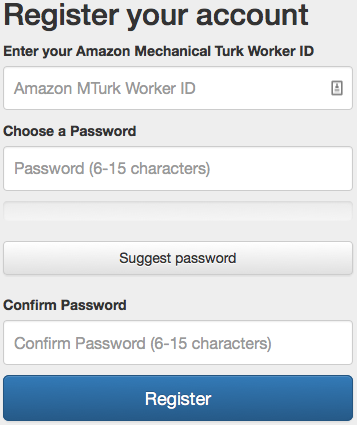
\includegraphics[width=\textwidth]{Images/1-register-meter}
            \caption{With strength meter}
            \label{fig:reg-str}
        \end{subfigure}
        ~
        \begin{subfigure}[t]{0.4\textwidth}
            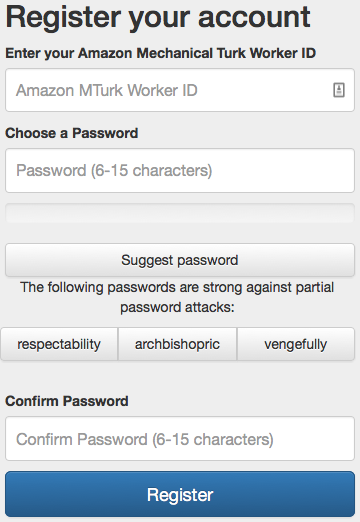
\includegraphics[width=\textwidth]{Images/1-register-meter-sugg}
            \caption{With strength meter and password suggestions}
            \label{fig:reg-str-sugg}
        \end{subfigure}
      }
      \caption{Registration page}\label{fig:registration}
    \end{figure}

  \section{Login page}
    \label{aps:login}
    \begin{figure}[H]
      \makebox[\textwidth][c] {
        \begin{subfigure}[t]{0.4\textwidth}
            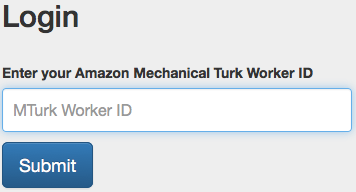
\includegraphics[width=\textwidth]{Images/2-login-init}
            \caption{Initial login screen}
            \label{fig:login-init}
        \end{subfigure}
        ~
        \begin{subfigure}[t]{0.4\textwidth}
            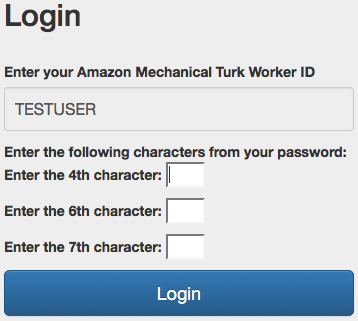
\includegraphics[width=\textwidth]{Images/2-login-ppass}
            \caption{Partial password challenge}
            \label{fig:login-ppass}
        \end{subfigure}
        ~
        \begin{subfigure}[t]{0.4\textwidth}
            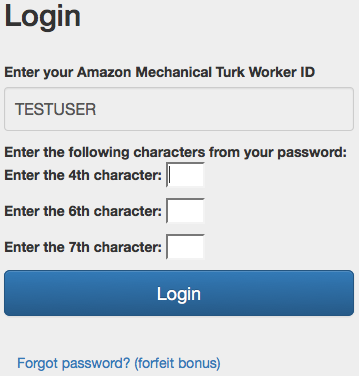
\includegraphics[width=\textwidth]{Images/2-login-ppass-forgot}
            \caption{Partial password challenge with ``Forgot password'' option}
            \label{fig:login-forgot}
        \end{subfigure}
      }
      \caption{Login page}\label{fig:login}
    \end{figure}

  \section{Completion page}
    \label{aps:complete}
    \begin{figure}[H]
      \centering
      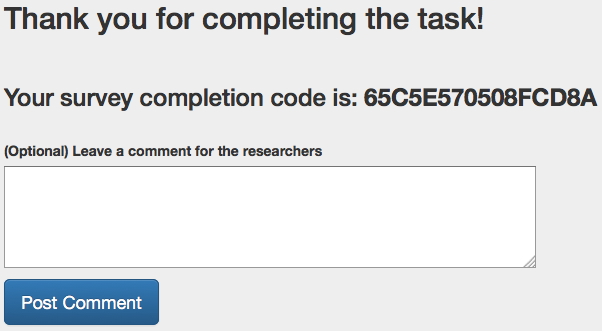
\includegraphics[width=\textwidth]{Images/3-success}
      \caption{Completion page}
      \label{fig:complete}
    \end{figure}